\documentclass{ctexart}
\usepackage[left=2.50cm, right=2.50cm, top=2.50cm, bottom=2.50cm]{geometry}

% -- text font --
% compile using Xelatex

%\setmainfont{Microsoft YaHei}  % 微软雅黑
%\setmainfont{YouYuan}  % 幼圆
%\setmainfont{NSimSun}  % 新宋体
%\setmainfont{KaiTi}    % 楷体
%\setmainfont{SimSun}   % 宋体
%\setmainfont{SimHei}   % 黑体

\usepackage{times}
%\usepackage{mathpazo}
%\usepackage{fourier}
%\usepackage{charter}
%\usepackage{helvet}

\usepackage{amsmath, amsfonts, amssymb} % math equations, symbols
\usepackage[english]{babel}
\usepackage{color}      % color content
\usepackage{graphicx}   % import figures
\usepackage{url}        % hyperlinks
\usepackage{bm}         % bold type for equations
\usepackage{multirow}
\usepackage{booktabs}
\usepackage{epstopdf}
\usepackage{epsfig}
\usepackage{algorithm}
\usepackage{algorithmic}
\usepackage{fancyhdr}   % 设置页眉、页脚
\usepackage{indentfirst}
\pagestyle{fancy}
\lhead{}
\chead{}
%\rhead{\includegraphics[width=1.2cm]{fig/ZJU_BLUE.eps}}
\lfoot{}
\cfoot{}
\rfoot{}

\usepackage{hyperref}   % bookmarks
\hypersetup{colorlinks, bookmarks, unicode} % unicode


\title{关于大数据的合理性的研究}
%\author{ 作者 Author \thanks{作者介绍 Brief introduction} }
\author{雷宇恒\ 蔡泽坤\ 谭欣雨}
\date{}

\begin{document}
    \maketitle
    %\thispagestyle{fancy}

\section{前言}
\subsection{大数据是什么}
\subsection{休谟问题是什么}
\subsection{两者是如何联系的}
\subsection{矛盾冲突点}
\subsection{理解、解决这个问题的重要意义}

\section{研究现状}
\subsection{随着大数据的发展的不同阶段,不同人对于这个问题的立场与观点是什么}
\subsection{现阶段学者对这个问题是如何认识的(分为主要几个阵营)}
\subsection{这些认识对于大数据的具体场景应用有什么具体的指导性作用、建议、引导吗}

\section{未来发展、研究方向展望}

大数据这个概念才提出不到30年,在这个期间还有很长一段时间收到当时计算机计算能力的限制而没有得到很好的发展。前几年大数据被重新提及,受到了世界各个学科的强烈关注,大数据技术也得到了飞速发展。大数据如今主要用途是在社会学,经济学与网络数据中寻求一些相关关系并对未来做出预测。目前来说,不同大数据的数据内容比较单一,都是限制在某一方面的有限变量,这对于大数据的预测有了很大的限制。在科学研究方面,目前人来在因果关系的环境下还不接受大数据带来的相关关系的理性理解,所以目前大数据并不能代替如今的研究方式。

目前在应用方面的发展方向是将不同的大数据整合,因为在不同大数据中的变量以及记录的信息是可以匹配起来的,这种匹配在技术方面是可行的,但是目前大数据是分属于不同公司或团体的财产,但是为了让大数据能够分析得出更综合的结论,必须将大数据的变量进行整合丰富。

在学科研究的方面,大数据需要一个合理的哲学解释,就是如何从大数据中的相关关系推断出因果关系。因为大数据有着数据量大,动态化,考虑全体样本的特性,大数据中的数据一定不是全部精准正确的,会有误差甚至是错误。有些观点认为现实世界中有因果关系的两个事物之间在某些因素的影响下也会产生误差甚至是错误,而一直延续至今的小样本(抽样)所得到的因果关系是在一个理想环境下得到的。所以在将来可能需要考虑现实情况下出现的干扰,而大数据是能够准确分析出来的。2008年,美国《连线》杂志主编克里斯(安德森),以 《理论的终结》为题发表论文,认为“有了足够的数据,数字自己会说话”,因而“相关关系足够了”。

休谟的问题实际上就是人类如何通过感觉经验性程普变规律性认识的问题。康德已经对此做出了一种回答,即是将这种因果关系判断为一种先天综合的描述,并且这种先天综合的描述是可以通过人们理性的分析得到的。但是康德还是最后还是没有办法指出哪些命题是先天的,哪些命题是综合的,在什么情况下这些命题是先天综合命题。而在大数据技术的影响下,我们通过大量的数据和动态的处理得到具有实时性质的相关关系在某些程度上是可以通过人类的理性分析得出的,这样的话对于休谟问题的将会有全新的解释方法。

若是能够解决大数据的相关关系能够解释休谟提出的问题,那么相当于能够得到大数据的相关关系可以推断出因果关系,从而将大数据中分析得到的结果作为一种理性知识。大数据将成为一种新的研究范式,因为大数据能够容纳错误,相比小样本的抽样实验,大数据不需要很高的自变量精度,同时大数据中量化的数据都是自动获取的,也排除了人为的偏好问题。大数据不但能解决现在科学研究范式能够解决的问题,也可以解决如今解决不了的复杂体系的问题。

对于大数据将来的发展,如果休谟问题能够被解决的话,大数据将会引发一场新的变革,成为下一代研究的新范式。

\subsection{大数据目前的发展方向是怎样的?}

大数据在当今时代主要用于对某些特定领域的问题智能化解决方案。当今所记录的数据类型集中在某一确定的领域内部,寻找在这一领域内部存在的相关性以及经验性的联系,根据这样的联系加以分析并提出具体的解决方案。在以往的科学研究中,大数据并没有展示出良好的应用,主要原因在于实验次数的受限,以及实验中存在的人为因素会影响到大数据中数据的自然性。不过目前在科学研究中,大数据依据自己经验的丰富性为科学提供了一种研究思路:利用大数据得出的相关性进行初步的解释,在通过一步一步的对其进行抽样、演绎推理和实验一步一步将这个相关性精确化。
\begin{figure}[htbp] 		
		\centering
		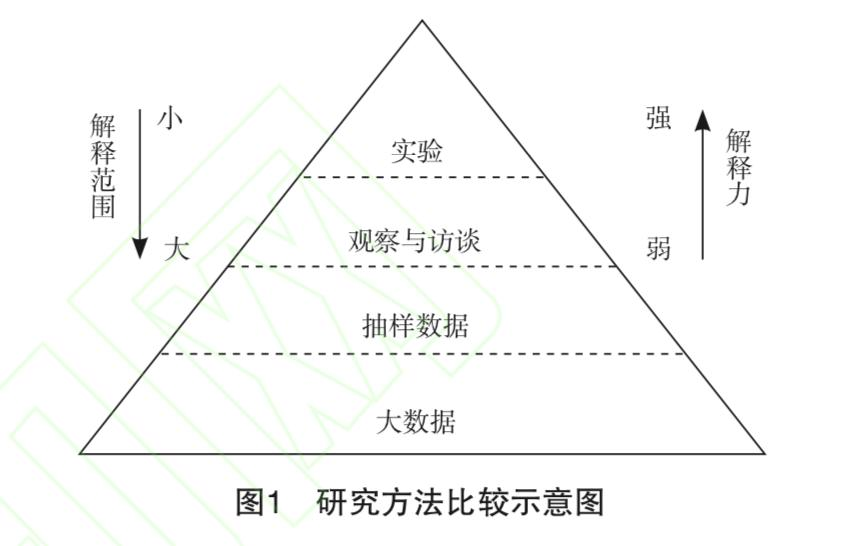
\includegraphics[scale=2,width=0.2\textwidth]{first.jpg}
		\caption{研究方法比较示意图}
		\label{first}		
\end{figure}

当今比较主流的发展方向分为社会学层面和科学研究层面:前者是将不同大数据的内容结合,形成多个大数据不同参数之间的联系,有利于进一步分析提供更加全局优化的结果。在科学研究中,大数据的发展就是突破目前人们认为大数据解释力小的约束,或是突破人类对局限认知世界可能性的观点。将来有机会将大数据应用到复杂性体系中取得相关性结果作为认知的可能。

\subsection{这样的发展趋势对解决这个问题有怎样的影响?}

休谟认为,因果律不是经验归纳可以证明的。利用大数据,我们便有可能将所有的可能性囊括在内,将所有的可能性进行经验性的归纳,使之成为因果关系。我们更有可能不能将所有可能性录入大数据中,但是通过一个比原来庞大丰富的多的经验归纳,我们是否可以理性的将相关性结果作为认知,这将会把休谟的问题抛开在一边,有些类似于康德的思想。

\subsection{休谟问题与大数据的冲突的解决的重要意义(restate)}

休谟问题与大数据冲突解决意味着将来通过大数据的分析我们依旧能够得到确切的知识,这就意味着将来的理论研究不需要通过演绎推理实现,而是可以通过大数据将实验结果的分析得到确认。将是一种彻底的科学研究的范式转换。

\section{结论}

    


    
    %\begin{figure}[htbp]
%		\centering
%		\includegraphics[width=0.2\textwidth]{fig/ZJU_BLACK.eps}
%		\includegraphics[width=0.2\textwidth]{fig/ZJU_BLUE.eps}
%		\caption{figure 1}		
%		\label{figure:zju1}
%	\end{figure}
%
%     Fig. \ref{figure:zju2}
%    \begin{figure}[htbp] 		
%		\centering
%		\includegraphics[width=0.2\textwidth]{fig/ZJU_BLACK.eps}
%		\includegraphics[width=0.2\textwidth]{fig/ZJU_BLUE.eps}
%		\caption{figure 2}
%		\label{figure:zju2}		
%	\end{figure}

\end{document}